\documentclass[
	12pt,
	a4paper,
	bibtotoc,
	cleardoubleempty, 
	idxtotoc,
	ngerman,
	openright
	final,
	listof=nochaptergap,
	]{scrbook}

\usepackage[T1]{fontenc}
\usepackage[utf8]{inputenc}

% ##################################################
% Unterstuetzung fuer die deutsche Sprache
% ##################################################
\usepackage{ngerman}
\usepackage[ngerman]{babel}
\usepackage{underscore}
% ##################################################
% Dokumentvariablen
% ##################################################

% Persoenliche Daten
\newcommand{\docA}{Eduard Albach}
\newcommand{\docB}{Felix Penthin}
\newcommand{\docC}{Marco Haas}
\newcommand{\docD}{Eric Saier}
\newcommand{\docE}{Philipp Schneider}

% Dokumentdaten
\newcommand{\docTitle}{Design Patterns in IBM Rhapsody}
%\newcommand{\docUntertitle}{} % Kein Untertitel
\newcommand{\docUntertitle}{UNTERTITEL}
% Arten der Arbeit: Bachelorthesis, Masterthesis, Seminararbeit, Diplomarbeit
\newcommand{\docArtDerArbeit}{Semesterprojekt}
%Studiengaenge: Allgemeine Informatik Bachelor, Computer Networking Bachelor,
% Software-Produktmanagement Bachelor, Advanced Computer Scinece Master
\newcommand{\docStudiengang}{STUDIENGANG}
\newcommand{\docAbgabedatum}{29.06.2015}
\newcommand{\docErsterReferent}{Prof. Dr. R. Müller}
%\newcommand{\docZweiterReferent}{-} % Wenn es nur einen Betreuer gibt
%\newcommand{\docZweiterReferent}{ZWEITER REFERENT}

% ##################################################
% Allgemeine Pakete
% ##################################################

% Abbildungen einbinden
\usepackage{graphicx}

% Zusaetsliche Sonderzeichen
\usepackage{dingbat}

% Farben
\usepackage{color}
\usepackage[usenames,dvipsnames,svgnames,table]{xcolor}

% Maskierung von URLs und Dateipfaden
\usepackage[hyphens]{url}

% Deutsche Anfuehrungszeichen
\usepackage[babel, german=quotes]{csquotes}

% Pakte zur Index-Erstellung (Schlagwortverzeichnis)
\usepackage{index}
\makeindex

% Ipsum Lorem
% Paket wird nur für das Beispiel gebraucht und kann gelöscht werden
\usepackage{lipsum}

% ##################################################
% Seitenformatierung
% ##################################################
\usepackage[
	portrait,
	bindingoffset=1.5cm,
	inner=2.5cm,
	outer=2.5cm,
	top=3cm,
	bottom=2cm,
	%includeheadfoot
	]{geometry}

% ##################################################
% Kopf- und Fusszeile
% ##################################################

\usepackage{fancyhdr}

\pagestyle{fancy}
\fancyhf{}
\fancyhead[EL,OR]{\sffamily\thepage}
\fancyhead[ER,OL]{\sffamily\leftmark}

\fancypagestyle{headings}{}

\fancypagestyle{plain}{}

\fancypagestyle{empty}{
  \fancyhf{}
  \renewcommand{\headrulewidth}{0pt}
}

%Kein "Kapitel # NAME" in der Kopfzeile
\renewcommand{\chaptermark}[1]{
	\markboth{#1}{}
   	\markboth{\thechapter.\ #1}{}
}

% ##################################################
% Schriften
% ##################################################

% Stdandardschrift festlegen
\renewcommand{\familydefault}{\sfdefault}

% Standard Zeilenabstand: 1,5 zeilig
\usepackage{setspace}
\onehalfspacing 

% Schriftgroessen festlegen
\addtokomafont{chapter}{\sffamily\large\bfseries} 
\addtokomafont{section}{\sffamily\normalsize\bfseries} 
\addtokomafont{subsection}{\sffamily\normalsize\mdseries} 
\addtokomafont{caption}{\sffamily\normalsize\mdseries} 

%Einrücken von Absätzen deaktivieren
\setlength{\parindent}{0pt}

% ##################################################
% Inhaltsverzeichnis / Allgemeine Verzeichniseinstellungen
% ##################################################

\usepackage{tocloft}

% Punkte auch bei Kapiteln
\renewcommand{\cftchapdotsep}{3}
\renewcommand{\cftdotsep}{3}

% Schriftart und -groesse im Inhaltsverzeichnis anpassen
\renewcommand{\cftchapfont}{\sffamily\normalsize}
\renewcommand{\cftsecfont}{\sffamily\normalsize}
\renewcommand{\cftsubsecfont}{\sffamily\normalsize}
\renewcommand{\cftchappagefont}{\sffamily\normalsize}
\renewcommand{\cftsecpagefont}{\sffamily\normalsize}
\renewcommand{\cftsubsecpagefont}{\sffamily\normalsize}

%Zeilenabstand in den Verzeichnissen einstellen
\setlength{\cftparskip}{.5\baselineskip}
\setlength{\cftbeforechapskip}{.1\baselineskip}

% ##################################################
% Abbildungsverzeichnis und Abbildungen
% ##################################################

\usepackage{caption}

\usepackage{wrapfig}

% Nummerierung von Abbildungen
\renewcommand{\thefigure}{\arabic{figure}}
\usepackage{chngcntr}
\counterwithout{figure}{chapter}

% Abbildungsverzeichnis anpassen
\renewcommand{\cftfigpresnum}{Abbildung }
\renewcommand{\cftfigaftersnum}{:}

% Breite des Nummerierungsbereiches [Abbildung 1:]
\newlength{\figureLength}
\settowidth{\figureLength}{\bfseries\cftfigpresnum\cftfigaftersnum}
\setlength{\cftfignumwidth}{\figureLength}
\setlength{\cftfigindent}{0cm}

% Schriftart anpassen
\renewcommand\cftfigfont{\sffamily}
\renewcommand\cftfigpagefont{\sffamily}

% ##################################################
% Tabellenverzeichnis und Tabellen
% ##################################################

% Nummerierung von Tabellen
\renewcommand{\thetable}{\arabic{table}}
\counterwithout{table}{chapter}

% Tabellenverzeichnis anpassen
\renewcommand{\cfttabpresnum}{Tabelle }
\renewcommand{\cfttabaftersnum}{:}

% Breite des Nummerierungsbereiches [Abbildung 1:]
\newlength{\tableLength}
\settowidth{\tableLength}{\bfseries\cfttabpresnum\cfttabaftersnum}
\setlength{\cfttabnumwidth}{\tableLength}
\setlength{\cfttabindent}{0cm}

%Schriftart anpassen
\renewcommand\cfttabfont{\sffamily}
\renewcommand\cfttabpagefont{\sffamily}

% Unterdrueckung von vertikalen Linien
\usepackage{booktabs}

%Fluss eigenschaften von Tabellen

\usepackage{float}

%Longtable

\usepackage{longtable}

% ##################################################
% Listings (Quellcode)
% ##################################################

\usepackage{listings}
\definecolor{codegreen}{rgb}{0,0.6,0}
\definecolor{codegray}{rgb}{0.5,0.5,0.5}
\definecolor{codepurple}{rgb}{0.58,0,0.82}
\definecolor{backcolour}{rgb}{0.95,0.95,0.92}
 
\lstdefinestyle{codestyle}{
    backgroundcolor=\color{backcolour},   
    commentstyle=\color{codegreen},
    keywordstyle=\color{magenta},
    numberstyle=\tiny\color{codegray},
    stringstyle=\color{codepurple},
    basicstyle=\footnotesize,
    breakatwhitespace=false,         
    breaklines=true,                 
    captionpos=b,                    
    keepspaces=true,                 
    numbers=left,                     
    numbersep=5pt,                  
    showspaces=false,                
    showstringspaces=false,
    showtabs=false,                  
    tabsize=2
}

\lstset{style=codestyle}

 \lstdefinelanguage{JavaScript}{
  keywords={break, case, catch, continue, debugger, default, delete, do, else, finally, for, function, if, in, instanceof, new, return, switch, this, throw, try, typeof, var, void, while, with},
  morecomment=[l]{//},
  morecomment=[s]{/*}{*/},
  morestring=[b]',
  morestring=[b]",
  sensitive=true
}	

% "define" Scala
\lstdefinelanguage{scala}{
  morekeywords={abstract,case,catch,class,def,%
    do,else,extends,false,final,finally,%
    for,if,implicit,import,match,mixin,%
    new,null,object,override,package,%
    private,protected,requires,return,sealed,%
    super,this,throw,trait,true,try,%
    type,val,var,while,with,yield},
  otherkeywords={=>,<-,<\%,<:,>:,\#,@},
  sensitive=true,
  morecomment=[l]{//},
  morecomment=[n]{/*}{*/},
  morestring=[b]",
  morestring=[b]',
  morestring=[b]"""
}
  	
% ##################################################
% Theoreme
% ##################################################
  	
% Umgebung fuer Beispiele
\newtheorem{beispiel}{Beispiel}

% Umgebung fuer These
\newtheorem{these}{These}

% Umgebung fuer Definitionen
\newtheorem{definition}{Definition}
  	
% ##################################################
% Literaturverzeichnis
% ##################################################

\usepackage{bibgerm}

% ##################################################
% Abkuerzungsverzeichnis
% ##################################################

\usepackage[printonlyused]{acronym}

% ##################################################
% PDF / Dokumenteninternelinks
% ##################################################

\usepackage[
	colorlinks=false,
   	linkcolor=black,
   	citecolor=black,
  	filecolor=black,
	urlcolor=black,
    bookmarks=true,
    bookmarksopen=true,
    bookmarksopenlevel=3,
    bookmarksnumbered,
    plainpages=false,
    pdfpagelabels=true,
    hyperfootnotes,
    pdftitle ={\docTitle},
    pdfauthor={\docA \docB \docC \docD},
    pdfcreator={\docA~\docB~\docC~\docD}]{hyperref}

\begin{document}

\setcounter{secnumdepth}{3}

% Titelblatt
\begin{titlepage}
\pagestyle{empty}

% ##################################################
% HFU-Logo einbinden
% ##################################################
\begin{flushright}
\begin{figure}[ht]
\flushright

\includegraphics[height=3cm]{content/pictures/hfu.jpg}
\end{figure}
\end{flushright}

% ##################################################
% Titel
% ##################################################
\begin{center}
{\fontsize{18}{22} \selectfont \docArtDerArbeit}\\[5mm]
\vspace{1cm}
\begin{onehalfspace}
{\fontsize{22}{26} \selectfont \textbf{\docTitle}}\\[5mm]


\end{onehalfspace}
\end{center}

% ##################################################
% Zusatzinformationen
% ##################################################
\vfill
\begin{center}
\begin{tabular}{lcl}
Betreuer  		&:& \docErsterReferent 	\\ \\
Vorgelegt am 	&:& \docAbgabedatum 	\\ \\
Vorgelegt von 	&:& \docA\\
				&&	\docB\\
				&&	\docC\\
				&&	\docD\\
				&&	\docE\\				
\end{tabular}
\end{center}
\end{titlepage}
\cleardoubleemptypage

\frontmatter


% Abstract
\chapter*{Abstract\markboth{Abstract}{}}
\addcontentsline{toc}{chapter}{Abstract}

[Englisches Abstract (100-120 Worte)]

[Deutsches Abstract (100-120 Worte)]
\cleardoubleemptypage

% Inhaltsverzeichnis test  2
\tableofcontents
\addcontentsline{toc}{chapter}{Inhaltsverzeichnis}
\cleardoubleemptypage

% Abbildungsverzeichnis einbinden und ins Inhaltsverzeichnis
% WORKAROUND: tocloft und KOMA funktionieren zusammen nicht
% korrekt\phantomsection
\addcontentsline{toc}{chapter}{\listfigurename} 
\listoffigures
\cleardoubleemptypage

% Tabellenverzeichnis einbinden und ins Inhaltsverzeichnis
% WORKAROUND: tocloft und KOMA funktionieren zusammen nicht
% korrekt\phantomsection
\phantomsection
\addcontentsline{toc}{chapter}{\listtablename}
\listoftables
\cleardoubleemptypage

% Abkürzungsverzeichnis
\chapter*{Abkürzungsverzeichnis\markboth{Abkürzungsverzeichnis}{}}
\addcontentsline{toc}{chapter}{Abkürzungsverzeichnis}

\begin{acronym}
\acro{HFU}{Hochschule Furtwangen University}
\end{acronym}

\mainmatter

\chapter{Einleitung}

\section{Aufgabenbeschreibung}

Ziel dieses Semesterprojektes ist es mit Rhapsody, einem Tool welches ein mächtiges Tool zur Codegenerierung ist, Design Pattern zu implementieren. Diese werden standardmäßig von Rhapsody nicht angeboten und sollen in Form von Stereotypen während diesem Semester implementiert und getestet werden.
\\
In dem vorangegangenen Semester wurde die Umsetzbarkeit der Design Pattern
\begin{itemize}
\item Singleton
\item Observer Pattern
\end{itemize}
belegt. Diese sollen nun dieses Semester vollständig umgesetzt und getestet werden. 
Sind diese Stereotypen dann vollständig in Rhapsody implementiert, ruft Rhapsody 
automatisch Java-Klassen auf, welche dann das als Objektbaum vorliegende Modell 
umbauen können.
\\
Sollte am Ende des Semesters noch genügend Zeit übrig sein, können
selbstverständlich noch weitere Design Pattern umgesetzt werden.



\include{content/designpattern}
\chapter{Singleton}

\section{Allgemeine Informationen}

\textit{Singleton} ist ein Entwurfsmuster das dafür sorgt, dass es nur eine Instanz einer Klasse gibt. Auf diese kann global zugegriffen werden und durch den privaten Konstruktor wird verhindert, dass andere Klassen weitere Instanzen erstellen können.
\\
\\
Die Singleton-Klasse umfasst daher einen privaten Konstruktor, einen Kopierkonstruktor, einen Zeiger auf die einzigartige Instanz und natürlich den Destruktor. Nur eine Methode ist öffentlich, die \textit{GetInstance}-Methode.
\\
\\
Es gibt viele verschiedene Implementierungen des Musters. Wir haben uns für diese Variante entschieden. Besonders muss zwischen zwei Versionen des Musters unterscheiden werden. Es gibt eine \textit{Eager Version} und eine \textit{Lazy Version}.
\\
\\
Bei der \textit{Eager Loading} Version findet das Erzeugen der Instanz beim Laden der Klasse statt. Vorteile sind hier die Einfachheit und die Threadsicherheit. Jedoch gibt es auch Nachteile. Durch eine verfrühte Erzeugung können Probleme entstehen. Wenn vor der Initialisierung Informationen benötigt werden kann es zu Problemen kommen. Auch eine zu frühe Erzeugung bei ressourcenintensiven Singleton-Klassen kann Probleme machen.
\\
\\
Man sieht, dass die Eager Loading Version nur dann sinnvoll ist, wenn es sich um eine kleine Singleton-Klasse handelt.
\\
\\
Gegenteilig verhält sich die \textit{Lazy Loading} Variante des Singleton Musters. Hier wird die Instanz erst beim ersten Aufruf erzeugt. Die Methode GetInstance überprüft, ob bereits eine Instanz erzeugt wurde und erstellt für den Fall, dass es keine gibt, eine neue. Falls es bereits eine Instanz gibt wird diese zurückgegeben.
\\
\\
Ein Problem bei dieser Methode ist die Threadsicherheit. Diese ist nicht mehr gegeben. \\

Es folgt ein Beispiel für eine Implementierung des Singleton Patterns von Scott Meyers, bei dem auch das Objekt beim Beenden des Programms zerstört wird:
\begin{lstlisting}

class Singleton
{
private:
    // Standard- und Copykonstruktor sowie Destruktor sind private. 
    // Nur Methoden dieser Klasse koennen auf sie 
    // zugreifen.
    Singleton() {};
    Singleton(const Singleton&);
    ~Singleton();

    // Es gibt nur eine Instanz. Jede Zuweisung waere
    // eine Selbstzuweisung.
    // Da Selbstzuweisungen selten Sinn machen, ist
    // der op= privat
    Singleton& operator=(const Singleton&);
public:
    // Diese statische Methode erzeugt die einzige
    // Instanz.
    // Nur ueber diese Methode erhalten Anwender den 
    // Zugriff auf die Instanz.
    static Singleton& GetInstance() 
    {
        // Die Instanz wird erst beim ersten Aufruf
        // erzeugt.
        // Endet das Programm, wird Instanz vernichtet.
        static Singleton Instance;
        return Instance;
    }
};
\end{lstlisting}

Natürlich kann man sich auch für eine andere Art von Singleton entscheiden, jedoch ist dies eine sehr einfache Art, das Singleton Pattern umzusetzen.
\cite{singelton}\cite{singelton2}
\section{Umsetzung}

Wenn der Entwickler ein UML-Diagramm in Rhapsody zeichnet und dabei eine bestimmte Klasse als Singleton implementieren möchte, setzt er bei dieser Klasse den Stereotype als Singleton. Möchte der Entwickler nun aus diesem Diagramm Code generieren, wird von Rhapsody wie in Kapitel 1 - Aufgabenbeschreibung erläutert Java-Klassen aufgerufen, die diese Klasse dann als Singleton-Klasse in C++-Code erzeugen. 
\\
Hierbei wird als erstes der Konstruktor und der Kopierkonstruktor auf private
gesetzt, da weder von \enquote{außerhalb} keine Instanz direkt über den
new-Operator erzeugt werden kann, noch ein Objekt kopiert werden soll. Möchte
man ein Objekt der Klasse anlegen, muss dies über die GetInstance-Methode
geschehen. In dieser Methode wird zunächst geprüft, ob es schon eine Instanz
gibt. Ist dies der Fall wird diese Instanz genutzt, wenn nicht wird eine neue Instanz erzeugt.\\


Falls der Nutzer eine Simplifizierung bei einem Projekt startet, bei welchem
bereits Code vorhanden ist, so wird zum einen überprüft, ob die
GetInstance-Methode oder das mInstance-Attribut vorhanden sind, zum anderen, ob
die Funktion/das Attribut von einer vorherigen Simplifizierung stammt. Ist dies
der Fall, wird die Simplifizierung normal durchgeführt und das Attribut bzw. die
Funktion überschrieben, da davon ausgegangen werden kann, dass der vorhandene
Code mit dem nun neu generierten übereinstimmt. \\
Sind Funktion oder Attribut vorhanden, aber stammen nicht aus einer vorherigen
Simplifizierung, wird ein Fehler generiert.


\chapter{Observer}

\section{Allgemein}
Das Observer Design Pattern (Beobachter Entwurfsmuster) gehört zu der Kategorie der behavioural 
patterns (Verhaltensmuster). Es wird verwendet, um die Änderung an dem Zustand eines Objekts zu
erfassen und alle davon abhängigen Objekte über die Änderung automatisch zu
informieren.\\
\newline
Die Funktionsweise des Observer Design Patterns erfordert zwei Arten von Objekten. Das Subject 
stellt Daten zur Verfügung und arbeitet fortlaufend mit diesen. Wurden diese Daten verändert
informiert das Subject seine Observer und teilt ihnen mit, dass sich der Objektzustand verändert 
hat. Der Observer kann anschließend auf diese Zustandsänderung reagieren.\\
\newline
Ein Beispiel für diesen Anwendungsfall ist eine grafische Oberfläche, welche
Daten anzeigt, die sich im laufenden Betrieb ändern können. Die grafische Oberfläche ist der Observer und die 
Klasse, welche die Daten zur Verfügung stellt, ist das Subject. Sobald sich nun
Daten ändern, wird der Observer vom Subject informiert und dieser kann anschließend die Daten auf der 
grafischen Oberfläche aktualisieren.\\
\newline

\begin{figure}[!htbp]
	\centering
	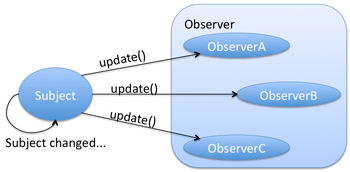
\includegraphics[width=0.66\textwidth]{content/pictures/Observer/observer01.png}
	\label{pic:bild}
	\caption{Observer Diagramm \cite{paulObserver}}
\end{figure}

Es gibt drei verschiedene Arten um diese Funktionalität umzusetzen, wobei jede ihre Vor- und 
Nachteile hat.\\ 
\newline
Push Notification\\
Bei der Push Notification benachrichtigen die Subjects ihre Observer nur dahingehend, dass 
sich etwas an dem Objektzustand verändert hat, aber nicht was für eine Veränderung das ist. 
Dadurch ist dies die schnellste Variante.\\
\newline
Push-Update Notification\\
Bei dieser Art der Umsetzung wird zusätzlich zu der Information über die Zustandsänderung
auch noch die geänderten Daten mitübertragen.\\
\newline
Pull Notification\\
Bei der Pull Notification informieren nicht die Subjects die Observer, sondern die Observer 
fragen in regelmäßigen Abständen bei den Subjects nach, ob Änderungen vorliegen.
Aufgrund des regelmäßigen Abfragens wird diese Variante seltener verwendet als die beiden anderen, da hier 
deutlich mehr Rechenzeit von der Observerfunktion benötigt wird.\\
\newline
Ein Nachteil des Observer Patterns ist der hohe Aufwand bei Änderungen am
Subject. Hier muss dann auch der Observer angepasst werden, was hohe Änderungskosten zur
Folge hat.\cite{wikiObserver}\\\\
Aufgrund der höheren Flexibilität wollen wir eine Push-Notification zum Einsatz bringen.

 \begin{lstlisting}
#include <list> 
#include "ObserverInterface.h" 
  
using namespace std; 
  
class Subject 
{ 
  
public: 
    void attach(ObserverInterface* observer); 
    void detach(ObserverInterface* observer); 
    void notify(); 
  
private: 
    list<ObserverInterface*> observers; 
  
  
protected: 
    // Durch protected-Konstruktor wird diese Klasse abstrakt 
    Subject() {}; 
  
};

// ObserverInterface.h // 
class ObserverInterface 
{ 
public: 
    virtual void update() = 0; 
};

// SubjectImpl.cpp // 
#include "Subject.h" 
#include "ObserverInterface.h" 
  
void Subject::attach(ObserverInterface* observer) 
{ 
    observers.push_back(observer); 
} 
  
  
void Subject::detach(ObserverInterface *observer) 
{ 
    observers.remove(observer); 
} 
  
  
void Subject::notify() 
{ 
    list<ObserverInterface*>::iterator iter = observers.begin(); 
    for ( ; iter != observers.end(); iter++ ) 
    { 
        (*iter)->update(); 
        
    }       
}

 // ConcreteSubject.h // 
#include <string> 
#include "Subject.h" 
  
using namespace std; 
  
class ConcrecteSubject : public Subject 
{ 
  
private: 
    string data; 
  
public: 
    void setData(string _data) { data = _data; } 
    string getData() { return data; } 
    ConcreteSubject() : Subject() {} 
};

 // ConcreteObserver.h // 
#include <string> 
#include "ObserverInterface.h" 
#include "ConcreteSubject.h" 
  
using namespace std; 
class ConcreteObserver : public ObserverInterface 
{ 
  
private: 
    string name; 
    string observerState; 
    ConcreteSubject* subject; // Dieses Objekt haelt die Daten (=notifier) 
  
public: 
    void update(); 
    void setSubject(ConcreteSubject* subj); 
    ConcreteSubject* getSubject(); 
    ConcreteObserver(ConcreteSubject* subj, string name); 
  
};


 // ConcreteObserverImpl.cpp // 
#include <iostream> 
#include "ConcreteObserver.h" 
  
using namespace std; 
  
  
// Daten anzeigen 
void ConcreteObserver::update() 
{ 
    observerState = subject->getData(); 
    cout << "Observer " << name << " hat neuen Zustand: " << observerState << endl; 
} 
  
void ConcreteObserver::setSubject(ConcreteSubject* obj) 
{ 
    subject = obj; 
} 
  
ConcreteSubject* ConcreteObserver::getSubject() 
{ 
    return subject; 
} 
  
  
ConcreteObserver::ConcreteObserver(ConcreteSubject* subj, string n) 
{ 
    name = n; 
    subject = subj; 
}

 // Main.cpp // 
#include "ObserverInterface.h" 
#include "ConcreteSubject.h" 
#include "ConcreteObserver.h" 
  
  
int main() 
{ 
  
    // Das Objekt haelt alle Daten (=notfier = subject) 
    ConcreteSubject* subj = new ConcretSubject(); 
    
    ObserverInterface* obs1 = new ConcreteObserver(subj,"A"); 
    ObserverInterface* obs2 = new ConcreteObserver(subj,"B"); 
  
    // Observer(=views) an Subjekt anhaengen (attachen) 
    subj->attach(obs1); 
    subj->attach(obs2); 
  
    // Daten aendern und Observer informieren (notify) 
    subj->setData("TestData"); 
    subj->notify(); 
  
       /* 
        Ausgabe: 
        Observer A hat neuen Zustand: TestData 
        Observer B hat neuen Zustand: TestData 
       */ 
  
    return 0; 
  
}

\end{lstlisting}

\section{Umsetzung}

Für die Umsetzung des Observer Design Pattern in Rhapsody wurden einige Richtlinien und 
Implementierungsdetails ausgearbeitet.\\
\newline
Für das Observer Design Pattern stehen zwei Stereotypen zur Verfügung. Zum einen der Observer 
und zum anderen das Subject. Wenn eine Klasse als Stereotyp Observer deklariert wird, wird das 
zugehörige Interface erstellt und in das bestehende Projekt eingefügt, mit dem Stereotyp Subject 
wird ebenso verfahren.\\
\newline
Um eine fehlerfreie Umsetzung zu realisieren wurde festgelegt, dass ein Benutzer im Lauf seiner 
Softwareentwicklung keine reservierten Klassen- und Methodennamen benutzen darf. Falls bereits Klassen existieren, die Observer/Subject heißen, muss überprüft werden, ob es sich dabei um unsere Implementierung aus einer früheren Simplification handelt oder ob der Nutzer diese selbst angelegt hat. Falls es sich um unsere Klassen handelt, soll ein Infotext ausgegeben werden; die Simplification soll die existierenden Klassen dann ignorieren und nicht überschreiben. Falls es sich um vom Nutzer angelegte Klassen handelt, soll eine Fehlermeldung ausgegeben und die Simplification abgebrochen werden.
Gleiches gilt für bereits implementierte Methoden. 
Diese Richtlinien werden bei der Übersetzung des Programms überprüft und im Fehlerfall 
entsprechende Fehlermeldungen generiert und die Übersetzung abgebrochen.\\
\newline
Das Observer Interface besitzt lediglich eine Methode update, welche als leere Methode 
implementiert wird. Das hat den Hintergrund, dass nicht ersichtlich ist wie auf Änderungen 
reagiert werden soll. Die Funktionalität muss vom Benutzer selbst festgelegt und implementiert 
werden.\\
\newline
Das Subject Interface besitzt drei öffentliche Methoden. Mit der Methode
\\ register_Observer können Observer für dieses Subject in eine Liste
hinzugefügt werden, und mit delete_Observer wieder entfernt. Diese zwei Methoden werden vom Interface automatisch vollständig zur Verfügung gestellt. Die Methode notify_Observer sendet eine Update-Benachrichtigung an die registrierten Observer.\\
\newline
Wird dieses Design Pattern verwendet, ist es zwar durchaus möglich dass ein Benutzer ein 
Observer ohne ein Subject implementiert (oder umgekehrt), jedoch macht die Verwendung 
dieser Stereotypen nur gemeinsam einen Sinn. In solch einem Fall soll das Programm zwar 
übersetzt werden, aber dennoch eine Warnung ausgegeben werden um den Benutzer darauf hinzuweisen.

						
\chapter{Guarded Call}

\section{Allgemeine Informationen}
Der "Guarded Call" ist ein Entwurfsmuster im Bereich der Nebenläufigkeit. Beim Guarded Call wird sichergestellt, dass der Code einer Methode nur von einem Thread gleichzeitig ausgeführt werden kann.\\
Dabei überprüft der Thread vor dem Aufruf der Methode ob sie bereits von einem anderen Thread gesperrt ist. Ist dies der Fall, wird der Thread auf den Zustand \enquote{schlafend} gesetzt und der Scheduler widmet sich einem anderen Thread zu. Ist die Methode allerdings nicht gesperrt setzt der aktive Thread die Sperre selbst, um anschließend die Methode auszuführen. Nachdem die Methode verlassen wurde, wird die Sperre wieder aufgehoben.\\
Wird bei der Methode ein Wert zurückgegeben, wird der Wert der Variable bzw. die Referenz des Objekts zunächst zwischengespeichert, um anschließend die Sperre aufzuheben und schließlich den gespeicherten Wert zurückzugeben.\\
Nachdem die Sperre aufgehoben wurde werden die schlafenden Threads aufgeweckt, wobei einer der Threads nun erneut die Sperre setzen und die Methode aufrufen kann.

\section{Umsetzung}
Anm: muss beim Meeting noch disktutiert werden:\\
1. ob das Mutex-Objekt evtl. von Rhapsody erstellt wird)\\
2. Funktionsnamen: myFunction (Benutzer) und myFunctionWrapper (generiert) oder myFunctionGuarded (Benutzer) und myFunction (generiert)\\

 \begin{lstlisting}
// (Funktion des Benutzers, die geschuetzt werden soll)
void myFunction() {

}

// (generierte Methode)
void myFunctionWrapper() {
	myFunctionMutex.lock();
	myFunction();
	myFunctionMutex.unlock();
}

bzw.

int myFunction2() {
	...
}

int myFunction2Wrapper() {
	myFunction2Mutex.lock();
	int temp = myFunction2();
	myFunction2Mutex.unlock();

	return temp;
}

\end{lstlisting}
\chapter{Tests}

In diesem Kapitel werden zu den drei Design Patterns die jeweiligen Testfälle erläutert.

\section{Singleton}

Um sicherzustellen, dass die Singleton-Klasse richtig implementiert worden ist, müssen neben dem Behandeln der Compiler-Fehler und Warnungen folgende Testfälle manuell überprüft werden: 

\begin{description}
  \item[1.] \hfill \\
  Als allererstes muss überprüft werden, ob der Standard-Konstruktor der Singleton-Klasse aufrufbar ist. Sollte dies der Fall sein, scheitert der Test, denn der Konstruktor sollte von außerhalb nicht aufrufbar, d.h. private sein.
  \item[2.] \hfill \\
  Weiterhin muss überprüft werden, ob man von einem bestehenden Singleton-Objekt eine Kopie erzeugen kann. Ist dies möglich, scheitert dieser Test, denn ein Singleton-Objekt darf nicht kopiert werden. Der Copy-Konstruktor muss auch private sein.
  \item[3.] \hfill \\
  Ein weiterer Test ist, dass geprüft werden muss, ob es möglich ist, ein Singleton-Objekt zur Laufzeit zu zerstören. Das Singelton-Objekt wird erst am Ende der Programmlaufzeit freigegeben. Kann das Objekt schon vorher zerstört werden, schlägt der Test fehl. Der Destruktor muss auch als private deklariert sein.
  \item[4.] \hfill \\
  Möchte man von außerhalb ein Objekt der Singleton-Klasse implementieren, muss dies über die einzige öffentliche Methode der Singleton-Klasse "GetInstance()" passieren. Hierbei wird ein neues Objekt angelegt, sofern noch keins vorhanden war, ansonsten wird einfach das "alte" Objekt zurückgegeben.
  \item[5.] \hfill \\
  Hat der Benutzer selbst eine GetInstance-Methode implementiert, muss Rhapsody bei der Erzeugung des Projektes einen Fehler ausgeben und die Erzeugung abbrechen.
  \item[6.] \hfill \\
  Nachdem das Singelton-Objekt mithilfe der getInstance()-Methode erzeugt wurde, liefert diese Methode stets die gleiche Instanz der Singleton-Klasse zurück. 
   
   
\end{description}

\section{Observer}

\section{Guarded Call}



\chapter{Implementierung}

In diesem Kapitel befindet sich der Quelltext des jeweiligen Pattern. Damit wird
nicht der Quelltext der Pattern gemeint, sondern die Umsetzung unserer
Simplification. Um eine eigene Simplification zu schreiben und auf die
Funktionen die Rhapsody bietet zu zugreifen, müssen einige Einstellungen
beachtet werden. Diese werden in der Dokumentation des Wintersemesters
erläutert. Da wir jedoch einige Anpassungen an den Pattern vorgenommen haben
konnten wir die User-Simplification des letzten Semesters nicht verwenden. 

\section{Singleton}
\lstinputlisting
    [caption={User-Simplification Singelton}
       \label{lst:javaclass},
       captionpos=t,language=JAVA]
 {content/pictures/HFUSingeltonSimplifier.java} 

\section{Observer}
Bei der Implentierung von Observer verlief zuerst alles nach Plan. Nach einiger
Zeit hat sich jedoch schnell gezeigt das wir unsere Implementierung nicht so wie
gedacht und gewünscht umsetzen können. Nach etlichen Stunden Arbeit mussten wir
hier das Design-Pattern Observer abbrechen bzw. schließen.\\
Da wir bei diesem Pattern zwei Klassen haben auf die, die Simplifizierung
Einfluss nimmt, hatten wir hier große Probleme.\\
Anfangs haben wir eine falsche Denkweiße verfolgt. Uns war nicht klar das die,
von Rhapsody gegebene, "onPostSimplification"-Methode für jede Klasse ausgeführt
wird.
Dies machte unseren Code nur sehr unübersichtlich und wir haben versucht in einem Durchlauf
beide Klassen, also die Observer- und Subject-Klassen in einem durchlauf
anzupassen. Durch langes Testen sind wir jedoch dahinter gekommen und haben
einen anderen Ansatz verfolgt.\\
Der andere Ansatz war, die erzeugten Klassen nach dem
gesetzten Sterotypen zu durchsuchen und nach der entsprechenden Klasse zu modifizieren.
Dies hat soweit auch funktioniert. Das Problem hierbei war der Typ "Observer". Egal ob
wir die Observer Objekte in eine Liste oder einen Vektor speichern. Wir müssen der 
Liste bzw. dem Vektor einen Typen zuweisen. Also was in diesen Behälter rein darf. Und
genau hier ist das Problem.\\
Dieses Problem wollten wir durch das Erzeugen einer Oberklasse "Observer" lösen.
Sieht nach einer einfachen Lösung aus, jedoch steckt der Teufel ja bekanntlich
im Detail. So war es auch in diesem Fall. Auch nach mehreren Stunden
Dokumentationen durch forschen und etwas experimentieren, haben wir keinen Weg
gefunden um eine Klasse zu erzeugen.\\
Natürlich bietet die API eine solche Funktion nur leider gibt es keine Beispiele
oder nähere Erklärung. So waren unsere Versuche eine Klasse zu erzeugen nicht
von Erfolg gekrönt. Selbst wenn das Implementieren der Klasse funktioniert
hätte, haben wir noch das Problem der Vererbung. Diese sollte natürlich auch
durch die Simplifizierung gelöst werden. Auch das, haben wir nicht aus den
gegebenen Dokumenten geschafft. Wir dachten uns dabei das der User einfach eine
Klasse erzeugen muss mit dem Namen Observer. Jedoch bringt das recht wenig, wenn
man hier noch zusätzlich die Vererbung herstellen muss.\\
So musste der User immer mehr der Simplifizierung übernehmen und das ist nun
wirklich nicht Sinn und Zweck einer solchen "automatischen" Simplifizierung.\\
\\
Ein anderes Problem waren die ganzen Imports. Verschiedene Bibliotheken müssen
inkludiert werden um einen problemlosen Ablauf sicherzustellen. Auch das sollte
nach Möglichkeit direkt bei der Simplifizierung geschehen. Das hat jedoch auch
nicht funktioniert. Somit hatten wir das Problem das der User mehr für die
Simplifizierung machen muss als die eigentliche Simplifizierung selbst. Somit
macht unsere Umsetzung hier wenig Sinn.\\
Dazu kam das wir am Observer-Pattern die von uns implementierte Fehlerbehandlung
testen sollten und auch eine Roundtrip-Kontrolle implementieren. Beides musste
von diesem Pattern abgezogen werden und am Singleton getestet werden. Weiter
unten im Text befindet sich eine ausführliche Beschreibung dazu.\\ \\
Nach Absprache mit dem Betreuer sind wir zu dem Entschluss gekommen das wir
dieses Design-Pattern hier abschließen und mit dem letzten der drei weiter machen.
Der bisher erzeugte Quellcode wird jedoch auch abgegeben, sodass auch zukünftige
Gruppen von diesen Erkenntnissen profitieren können.

\section{Guarded Call}

\section{Fehlerbehandlung}

\subsection{Allgemein}
Besitzt eine Benutzerklasse ungültigen Code für das ausgewählte Design Pattern (bspw. eine 
bereits vorhandene, vom Benutzer erstellte getInstance Methode beim Singleton Design Pattern) 
sollte der Code-Generierungsprozess abgebrochen werden. Dabei wird die \textit{TBD} Methode der 
Klasse AbstractSimplifier aufgerufen, bei welcher fehlerhafter C++ Code generiert wurde, wodurch 
wiederum Rhapsody gezwungen wird den Simplification-Prozess abzubrechen.

\section{Roundtrip}


\section{Ungültige Benutzerklasse}

\chapter{Installation}
In diesem Kapitel gehen wir auf die Installation der Simplifizierung ein. Da
dieses Projekt auch in zukünftigen Projekten verwendet werden soll muss eine
Installationsbeschreibung vorhanden sein. Diese soll dem Administrator eine
einfache Installation ermöglichen.\\
Die Installation sollte nur von einem Administrator durchgeführt werden.
Natürlich wird eine ordentliche Installation von Rhapsody vorausgesetzt. Der
Rest lässt sich grob Grob in drei Punkte aufteilen.
Dazu gehören:
\begin{itemize}
  \item Installation von Eclipse (Optional)
  \item Anpassen der hep Datei
  \item Projekte richtig anlegen bzw. einbinden.
\end{itemize}
Der Installationsort für Eclipse und die Version ist hierbei egal. Eigentlich
wird Eclipse nur benötigt um die User-Simplifizierung zu bauen. Die benötigten
Dateien legt Eclipse standardmäßig in einem "bin" Ordner ab. Dieser Ordner ist
wichtig. Aus diesem Ordner werden die Dateien gelesen und Rhapsody erstellt
unsere Pattern. Bei unseren Projekten befindet sich das Rhapsody-Projekt im
Eclipse Workspace.
\begin{figure}[!htbp]
	\centering
	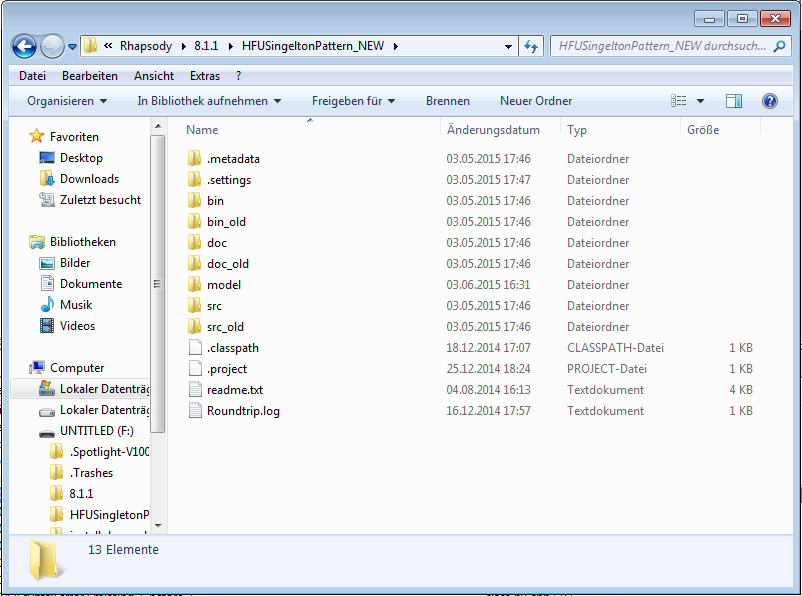
\includegraphics[width=0.79\textwidth]{content/pictures/install/struktur.png}
	\label{pic:bild}
	\caption{Ordnerstruktur von Eclipse-Workspace}
\end{figure}
Im Ordner model befindet sich das jeweilige Rhapsody-Projekt. Dies ist nicht
zwingend, jedoch haben wir so alle Projekte angelegt. Damit Rhapsody jetzt auch
weiß das wir eine User-Simplifizierung haben, muss die hep Datei angepasst
werden. Diese befindet sich im model-Ordner und in dem jeweiligen angelegten
Projekt mit der Endung _rpy.
\begin{figure}[!htbp]
	\centering
	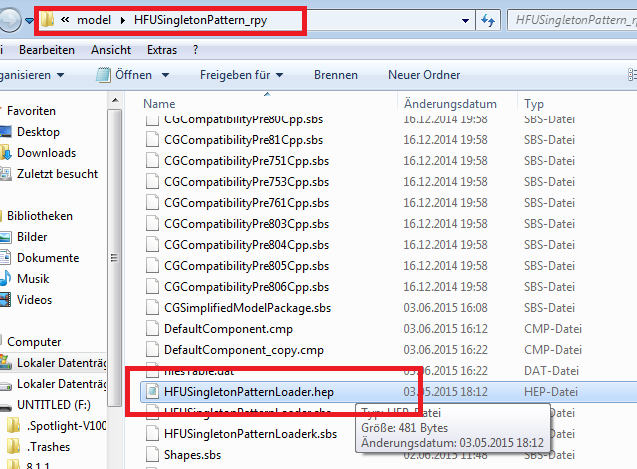
\includegraphics[width=0.88\textwidth]{content/pictures/install/model.png}
	\label{pic:bild}
	\caption{Erstelltes Projektverzeichniss}
\end{figure}
Die .hep Datei kann mit einem Texteditor geöffnet werden und angepasst werden.
In unserem Fall sieht diese folgendermaßen aus.
\begin{figure}[!htbp]
	\centering
	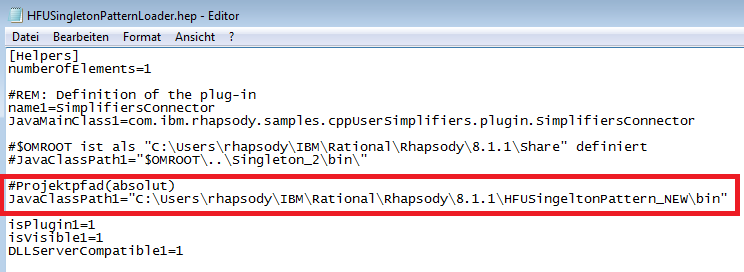
\includegraphics[width=0.88\textwidth]{content/pictures/install/hep.png}
	\label{pic:bild}
	\caption{Hep Datei}
\end{figure}
Hierbei interessiert uns nur die rote Markierung. Hier sieht man auch den
anfangs erwähnten bin Ordner.\\
Da aber auch in zukünftigen Projekten auf diese User-Simplifizierung zugegriffen
werden soll, ist es sinnvoll auch Eclipse zu installieren. Hier kann dann ganz
einfach die Simplifizierung angepasst werden. Da es hier keine main-Funktion
gibt, gibt es auch keinen ausführbaren Code. Eclipse erstellt durch das
Speichern der Dateien die .class Dateien, die wiederum im bin Ordner des
Projekts landen.\\ 
\textbf{WICHTIG}\\
Fals die Implementierung angepasst bzw. geändert wird, muss
Rhapsody beendet werden und erneut gestartet werden. Erst jetzt ist die Änderung
wirksam.  
\begin{figure}[!htbp]
	\centering
	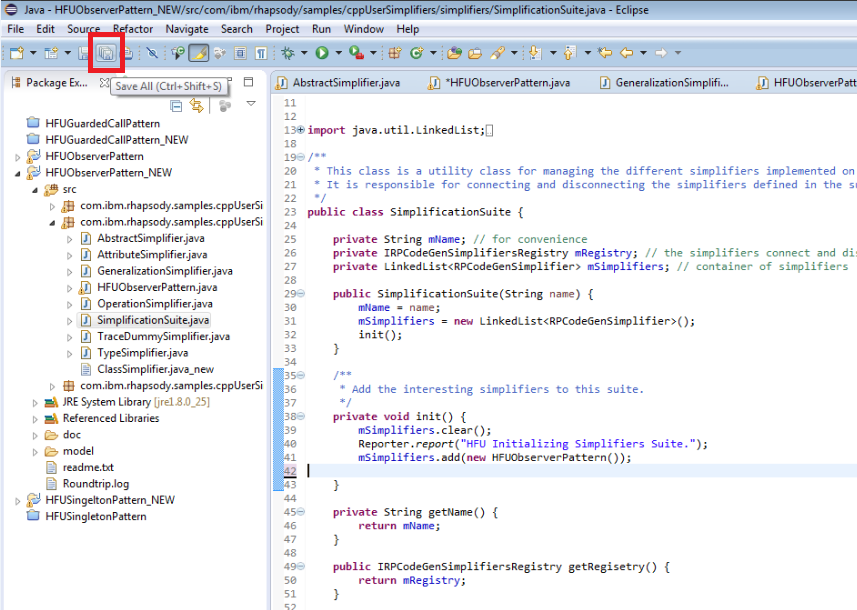
\includegraphics[width=0.95\textwidth]{content/pictures/install/saveBin.png}
	\label{pic:bild}
	\caption{Speichern und Erstellen der .class Dateien}
\end{figure}





%\chapter{Ausblick}
%\chapter{Fazit}

% Schalgwortverzeichnis (Index)
%\printindex

% Literaturverzeichnis
\singlespacing
\bibliographystyle{alphadin}
\bibliography{bibtex}

% Eidesstattliche Erklärung
\chapter*{Eidesstattliche Erklärung\markboth{Eidesstattliche Erklärung}{}}
% Eintrag in das Inhaltsverzeichnis 
\addcontentsline{toc}{chapter}{Eidesstattliche Erklärung}

Ich versichere, dass ich die vorstehende Arbeit selbständig verfasst und hierzu
keine anderen als die angegebenen Hilfsmittel verwendet habe. Alle Stellen der Arbeit die 
wörtlich oder sinngemäß aus fremden Quellen entnommen wurden, sind als solche kenntlich gemacht.
\\
\\
Die Arbeit wurde bisher in gleicher oder ähnlicher Form in keinem anderen
Studiengang als Prüfungsleistung vorgelegt oder an anderer Stelle
veröffentlicht.
\\
\\
Ich bin mir bewusst, dass eine falsche Erklärung rechtliche Folgen haben kann.

\vspace*{1.5cm} \par
\line(1,0){200} \par
%\docOrt, den  \docAbgabedatum ~~\docVorname~\docNachname

\appendix
% Hier können Anhaenge angefuegt werden

\end{document}      